\documentclass[usenames,dvipsnames,aspectratio=169]{beamer}
\usepackage{../common/cpp}

\title[OO Programozás - C++]{OO Programozás}
\subtitle{Konstansok}

\begin{document}

%1
\begin{frame}[plain]
  \titlepage
  \logoalul
\end{frame}

\section{Konstansok}

\subsection{\texttt{const}}

\begin{frame}
    A \texttt{const} típusmódosító változókkal használva
    \begin{itemize}
        \footnotesize
        \item \emph{Konstans változó} (\kiemel{paradoxon!} $\to$ \emph{elnevezett konstans})
        \item Memóriában helyezik el,
        \item azonnali inicializálást igényel, 
        \item értéke megjelenik a nyomkövető programokban (debugger),
        \item csak olvasható (fordító biztosítja),
        \item van típusa (vö. \texttt{\#define}).
        \item Láthatóságuk, hatókörük jobban szabályozható.
    \end{itemize}
    \vfill
    Tömbök definiálása, méret megadása
    \begin{itemize}
        \footnotesize
        \item konstans kifejezéssel,
        \item konstans kifejezéssel inicializált elnevezett konstanssal,
        \item vagy tetszőleges kifejezéssel C99 / C++14-től
    \end{itemize}
\end{frame}

\begin{frame}
    \begin{exampleblock}{\textattachfile{constMain.cpp}{constMain.cpp}}
        \lstinputlisting[language=C++,linerange={1-11},numbers=left,firstnumber=1]{constMain.cpp}
    \end{exampleblock}
\end{frame}

\begin{frame}
    \begin{exampleblock}{\textattachfile{constMain.cpp}{constMain.cpp}}
        \small
        \lstinputlisting[language=C++,linerange={12-24},numbers=left,firstnumber=12]{constMain.cpp}
    \end{exampleblock}
\end{frame}

\begin{frame}
    \begin{exampleblock}{\textattachfile{constHeader.h}{constHeader.h}}
        \lstinputlisting[language=C++,linerange={1-3},numbers=left,firstnumber=1]{constHeader.h}
    \end{exampleblock}
    \begin{exampleblock}{\textattachfile{constSource.cpp}{constSource.cpp}}
        \lstinputlisting[language=C++,linerange={1-1},numbers=left,firstnumber=1]{constSource.cpp}
    \end{exampleblock}
\end{frame}

\subsection{\texttt{constexpr}}

\begin{frame}
    A \texttt{constexpr} módosító (C++11/14) hatása a függvényekre:
    \begin{itemize}
        \item ,,Értékeld ki fordításkor!'' $\to$ gyorsabb programok, lassabb fordítás
        \item Viszonylag egyszerű függvények készíthetők csak vele (C++11: csak 1 utasítás)
        \item Csak olyan globális változókra hivatkozhat, melyek konstansok
        \item Csak \texttt{constexpr} függvényt hívhat, akár önmagát is
        \item Értékkel kell visszatérnie
        \item Nem csak konstansokkal ,,hívható'', de akkor az eredmény nem használható konstans inicializálására
        \item C++11-ben még tiltott volt a prefix $++$ operátor használata
    \end{itemize}
\end{frame}

\begin{frame}
    \begin{exampleblock}{\textattachfile{constexpr.cpp}{constexpr.cpp}}
        \scriptsize
        \lstinputlisting[language=C++,linerange={3-17},numbers=left,firstnumber=3]{constexpr.cpp}
    \end{exampleblock}
\end{frame}

\begin{frame}[fragile]
    \begin{exampleblock}{\textattachfile{fibonacci1.cpp}{fibonacci1.cpp}}
        \scriptsize
        \vspace{-.2cm}
        \lstinputlisting[language=C++,linerange={3-10},numbers=left,firstnumber=3]{fibonacci1.cpp}
        \vspace{-.2cm}
    \end{exampleblock}
    \begin{block}{Mérés}
        \vspace{-.4cm}
        \scriptsize
        \begin{verbatim}
$ time ./fibonacci1
2178309

real	0m0,005s
user	0m0,005s
sys	0m0,000s    
\end{verbatim}
        \vspace{-.4cm}
    \end{block}
\end{frame}

\begin{frame}[fragile]
    \begin{exampleblock}{\textattachfile{fibonacci2.cpp}{fibonacci2.cpp}}
        \scriptsize
        \vspace{-.2cm}
        \lstinputlisting[language=C++,linerange={3-10},numbers=left,firstnumber=3]{fibonacci2.cpp}
        \vspace{-.2cm}
    \end{exampleblock}
    \begin{block}{Mérés}
        \vspace{-.4cm}
        \scriptsize
        \begin{verbatim}
$ time ./fibonacci2
2178309

real	0m0,036s
user	0m0,036s
sys	0m0,000s            
\end{verbatim}
        \vspace{-.4cm}
    \end{block}
\end{frame}

\begin{frame}
    Osztályok tagfüggvényei, sőt, konstruktor is jelölhető \texttt{constexpr}-nek, de
    \begin{itemize}
        \item Az adattagok kvázi konstansok lesznek, amik inicializálása túl későn van a konstruktorban $\to$ \emph{taginicializáló lista}
        \item Konstans adattagok és referenciák csak taginicializáló listával hozhatók létre.
        \item Ez egyébként használható lett volna a nem konstans adattagok inicializálására is.
        \item Példányosításkor a paramétereknek konstansnak kell lenniük.
        \item A tagfüggvények implicit inline-ok lesznek.
    \end{itemize}
\end{frame}

\begin{frame}
    \begin{exampleblock}{\textattachfile{Rectangle10.cpp}{Rectangle10.cpp}}
        \scriptsize
        \lstinputlisting[language=C++,linerange={3-17},numbers=left,firstnumber=3]{Rectangle10.cpp}
    \end{exampleblock}
\end{frame}

\begin{frame}
    \begin{exampleblock}{\textattachfile{Rectangle10.cpp}{Rectangle10.cpp}}
        \scriptsize
        \lstinputlisting[language=C++,linerange={19-24},numbers=left,firstnumber=19]{Rectangle10.cpp}
    \end{exampleblock}
\end{frame}


\subsection{Konstansok és mutatók}

\begin{frame}
    Mutató konstans változóra:
    \begin{itemize}
        \item Maga a mutató nem konstans, nem \emph{kell} inicializálni.
        \item Mutathat változóra, csak olvashatóvá téve azt.
    \end{itemize}
    \begin{exampleblock}{\textattachfile{constptr.cpp}{constptr.cpp}}
        \scriptsize
        \lstinputlisting[language=C++,linerange={5-11},numbers=left,firstnumber=5]{constptr.cpp}
    \end{exampleblock}
\end{frame}

\begin{frame}
    Mutató változóra:
    \begin{itemize}
        \item Nem tartalmazhatja elnevezett állandó címét, mert a védelem nem kerülhető meg.
    \end{itemize}
    \begin{exampleblock}{\textattachfile{constptr.cpp}{constptr.cpp}}
        \scriptsize
        \lstinputlisting[language=C++,linerange={14-15},numbers=left,firstnumber=14]{constptr.cpp}
    \end{exampleblock}
\end{frame}

\begin{frame}
    Konstans mutató egy változóra:
    \begin{itemize}
        \item Mivel a mutató konstans, inicializálni kell.
        \item A mutatott változó módosítható, de a mutató nem mutathat máshova.
    \end{itemize}
    \begin{exampleblock}{\textattachfile{constptr.cpp}{constptr.cpp}}
        \scriptsize
        \lstinputlisting[language=C++,linerange={18-21},numbers=left,firstnumber=18]{constptr.cpp}
    \end{exampleblock}
\end{frame}

\begin{frame}
    Konstans mutató konstansra:
    \begin{itemize}
        \item Mindent csak olvasni lehet.
        \item Kiolvasás hátulról előre:\\ \emph{cpci} egy \emph{const} mutató (\emph{*}), ami olyan \emph{int}-et címez, ami \emph{const}.
    \end{itemize}
    \begin{exampleblock}{\textattachfile{constptr.cpp}{constptr.cpp}}
        \scriptsize
        \lstinputlisting[language=C++,linerange={24-26},numbers=left,firstnumber=24]{constptr.cpp}
    \end{exampleblock}
\end{frame}

\subsection{Konstansok és referenciák}

\begin{frame}
    Referencia konstansra:
    \begin{itemize}
        \item Minden referenciát inicializálni kell.
        \item Ha változót rendelünk hozzá, akkor az érték ezen keresztül csak olvasható lesz.
        \item Inicializálható konstans kifejezéssel!
    \end{itemize}
    \begin{exampleblock}{\textattachfile{constref.cpp}{constref.cpp}}
        \scriptsize
        \lstinputlisting[language=C++,linerange={5-11},numbers=left,firstnumber=5]{constref.cpp}
    \end{exampleblock}
\end{frame}

\begin{frame}
    A referenciák mindig konstansok.
    \begin{exampleblock}{\textattachfile{constref.cpp}{constref.cpp}}
        \scriptsize
        \lstinputlisting[language=C++,linerange={14-14},numbers=left,firstnumber=14]{constref.cpp}
    \end{exampleblock}
    \vfill
    Nem kerülhető meg a védelem konstansot címző nem konstans referenciával.
    \begin{exampleblock}{\textattachfile{constref.cpp}{constref.cpp}}
        \tiny
        \lstinputlisting[language=C++,linerange={17-17},numbers=left,firstnumber=17]{constref.cpp}
    \end{exampleblock}
\end{frame}

\subsection{Konstansok és függvények}

\begin{frame}
    Ha a függvény paramétere konstans, akkor a fv.-en belül sem változtatható meg az értéke, de a hívót ez nem érdekli (érték szerinti paraméterátadás). \\
    De ha a paraméter mutató vagy referencia, akkor a fv. megváltoztathatná a változó értékét!
    \begin{exampleblock}{\textattachfile{constfn.cpp}{constfn.cpp}}
        \small
        \lstinputlisting[language=C++,linerange={3-9},numbers=left,firstnumber=3]{constfn.cpp}
    \end{exampleblock}
\end{frame}

\begin{frame}
    \begin{exampleblock}{\textattachfile{constfn.cpp}{constfn.cpp}}
        \scriptsize
        \lstinputlisting[language=C++,linerange={11-17},numbers=left,firstnumber=11]{constfn.cpp}
        \lstinputlisting[language=C++,linerange={39-45},numbers=left,firstnumber=39]{constfn.cpp}
    \end{exampleblock}
\end{frame}

\begin{frame}
    Ha a visszatérési érték típusa alaptípus, nincs haszna a \texttt{const}-nak (nem balérték). \\
    De ha mutató vagy referencia, a visszatérési érték megváltoztatása tiltható \texttt{const}-tal.
    \begin{columns}[T]
        \begin{column}{0.45\textwidth}
            \begin{exampleblock}{\textattachfile{constfn.cpp}{constfn.cpp}}
                \small
                \lstinputlisting[language=C++,linerange={19-27},numbers=left,firstnumber=19]{constfn.cpp}
            \end{exampleblock}
        \end{column}
        \begin{column}{0.45\textwidth}
            \begin{exampleblock}{\textattachfile{constfn.cpp}{constfn.cpp}}
                \small
                \lstinputlisting[language=C++,linerange={29-37},numbers=left,firstnumber=29]{constfn.cpp}
            \end{exampleblock}
        \end{column}
    \end{columns}
\end{frame}

\begin{frame}
    \begin{exampleblock}{\textattachfile{constfn.cpp}{constfn.cpp}}
        \small
        \lstinputlisting[language=C++,linerange={39-39},numbers=left,firstnumber=39]{constfn.cpp}
        \lstinputlisting[language=C++,linerange={46-50},numbers=left,firstnumber=46]{constfn.cpp}
    \end{exampleblock}
\end{frame}

\subsection{Konstansok és objektumok}

\begin{frame}
    Példány is lehet konstans. Az adattagok többnyire eleve rejtettek, ezért kívülről nem írhatók. Nyilvános, konstans tag: getter elhagyható.\\
    Konstans tagfüggvény konstans objektumon is hívható!
    \begin{exampleblock}{\textattachfile{Rectangle11.cpp}{Rectangle11.cpp}}
        \small
        \lstinputlisting[language=C++,linerange={3-10},numbers=left,firstnumber=3]{Rectangle11.cpp}
    \end{exampleblock}
\end{frame}

\begin{frame}
    \begin{exampleblock}{\textattachfile{Rectangle11.cpp}{Rectangle11.cpp}}
        \scriptsize
        \lstinputlisting[language=C++,linerange={12-27},numbers=left,firstnumber=12]{Rectangle11.cpp}
    \end{exampleblock}
\end{frame}

\begin{frame}
    Konstans tagfüggvény is módosíthat egy adattagot, ha az \texttt{mutable}. Cél: érdemi állapotváltozást nem jelentő változások, pl. gyorsítótárak menedzselése.
    \begin{exampleblock}{\textattachfile{Rectangle12.cpp}{Rectangle12.cpp}}
        \lstinputlisting[language=C++,linerange={3-10},numbers=left,firstnumber=3]{Rectangle12.cpp}
    \end{exampleblock}
\end{frame}

\begin{frame}
    \begin{exampleblock}{\textattachfile{Rectangle12.cpp}{Rectangle12.cpp}}
        \scriptsize
        \lstinputlisting[language=C++,linerange={12-22},numbers=left,firstnumber=12]{Rectangle12.cpp}
    \end{exampleblock}
    (Sajnos) néhány további kivételes helyzetben is módosíthatja a \texttt{const} tagfüggvény a példány állapotát, pl.
    a tag struktúrát nem lehet lecserélni, de annak tagját már lehet módosítani (tranzitívan).
\end{frame}

\subsection{Beágyazott objektumok inicializálása}

\begin{frame}
    Egy objektumnak lehet beágyazott objektuma, ami szintén a taginicializáló listán keresztül inicializálható. Ha ezt nem tesszük meg $\to$ alapértelmezett konstruktor hívása, ha van ilyen.
    \begin{exampleblock}{\textattachfile{Rectangle13.cpp}{Rectangle13.cpp}}
        \lstinputlisting[language=C++,linerange={4-10},numbers=left,firstnumber=4]{Rectangle13.cpp}
    \end{exampleblock}
\end{frame}

\begin{frame}
    \begin{exampleblock}{\textattachfile{Rectangle13.cpp}{Rectangle13.cpp}}
        \scriptsize
        \lstinputlisting[language=C++,linerange={12-26},numbers=left,firstnumber=12]{Rectangle13.cpp}
    \end{exampleblock}
\end{frame}

\begin{frame}
    \begin{exampleblock}{\textattachfile{Rectangle13.cpp}{Rectangle13.cpp}}
        \small
        \lstinputlisting[language=C++,linerange={28-32},numbers=left,firstnumber=28]{Rectangle13.cpp}
    \end{exampleblock}
\end{frame}

\section{Származtatás, absztrakt osztályok, interfészek}

\subsection{Gyorsítótárazott síkidomok}

\begin{frame}
    Induljunk ki \textattachfile{Rectangle12.cpp}{Rectangle12}-ből, de 
    \begin{itemize}
        \item a kerület/terület lekérdezést (minden síkidomnál hasonlóan elvégezhető tevékenység) válasszuk külön a számítások elvégzésétől,
        \item a méretek legyenek módosíthatóak, és
        \item készítsünk háromszög (\texttt{Triangle}) osztályt is!
    \end{itemize}
\end{frame}    
     
\begin{frame}
    \begin{columns}[T]
        \column{.5\textwidth}
            \begin{exampleblock}{\textattachfile{Rectangle14.h}{Rectangle14.h}}
                \scriptsize
                \lstinputlisting[language=C++,linerange={4-10},numbers=left,firstnumber=4]{Rectangle14.h}
            \end{exampleblock}
        \column{.5\textwidth}
            \begin{exampleblock}{\textattachfile{Triangle14.h}{Triangle14.h}}
                \scriptsize
                \lstinputlisting[language=C++,linerange={6-11},numbers=right,firstnumber=6]{Triangle14.h}
            \end{exampleblock}
    \end{columns}
\end{frame}

\begin{frame}
    \begin{columns}[T]
        \column{.5\textwidth}
            \begin{exampleblock}{\textattachfile{Rectangle14.h}{Rectangle14.h}}
                \scriptsize
                \lstinputlisting[language=C++,linerange={11-22},numbers=left,firstnumber=11]{Rectangle14.h}
            \end{exampleblock}
        \column{.5\textwidth}
            \begin{exampleblock}{\textattachfile{Triangle14.h}{Triangle14.h}}
                \scriptsize
                \lstinputlisting[language=C++,linerange={12-23},numbers=right,firstnumber=12]{Triangle14.h}
            \end{exampleblock}
    \end{columns}
\end{frame}

\begin{frame}
    \begin{columns}[T]
        \column{.5\textwidth}
            \begin{exampleblock}{\textattachfile{Rectangle14.h}{Rectangle14.h}}
                \scriptsize
                \lstinputlisting[language=C++,linerange={23-33},numbers=left,firstnumber=23]{Rectangle14.h}
            \end{exampleblock}
        \column{.5\textwidth}
            \begin{exampleblock}{\textattachfile{Triangle14.h}{Triangle14.h}}
                \scriptsize
                \lstinputlisting[language=C++,linerange={24-34},numbers=right,firstnumber=24]{Triangle14.h}
            \end{exampleblock}
    \end{columns}
\end{frame}

\begin{frame}
    \begin{columns}[T]
        \column{.5\textwidth}
            \begin{exampleblock}{\textattachfile{Rectangle14.cpp}{Rectangle14.cpp}}
                \fontsize{7}{8} \selectfont
                \lstinputlisting[language=C++,linerange={3-6},numbers=left,firstnumber=3]{Rectangle14.cpp}
                \lstinputlisting[language=C++,linerange={13-19},numbers=left,firstnumber=13]{Rectangle14.cpp}
                \lstinputlisting[language=C++,linerange={29-31},numbers=left,firstnumber=29]{Rectangle14.cpp}
            \end{exampleblock}
        \column{.5\textwidth}
        \begin{exampleblock}{\textattachfile{Triangle14.cpp}{Triangle14.cpp}}
            \fontsize{7}{8} \selectfont
            \lstinputlisting[language=C++,linerange={3-6},numbers=left,firstnumber=3]{Triangle14.cpp}
            \lstinputlisting[language=C++,linerange={18-24},numbers=left,firstnumber=18]{Triangle14.cpp}
            \lstinputlisting[language=C++,linerange={34-38},numbers=left,firstnumber=34]{Triangle14.cpp}
        \end{exampleblock}
    \end{columns}
\end{frame}

\begin{frame}[fragile]
    \begin{exampleblock}{\textattachfile{main14.cpp}{main14.cpp}}
        \vspace{-.2cm}
        \fontsize{7}{8} \selectfont
        \lstinputlisting[language=C++,linerange={2-15},numbers=left,firstnumber=2]{main14.cpp}
        \vspace{-.2cm}
    \end{exampleblock}
    \begin{block}{Kimenet}
        \vspace{-.4cm}
        \fontsize{7}{8} \selectfont
        \begin{verbatim}
Rectangle #1 Area: 2 Perimeter: 6
Rectangle #2 Area: 6 Perimeter: 10
Rectangle #3 Area: 12 Perimeter: 14
        \end{verbatim}
        \vspace{-.4cm}
    \end{block}
\end{frame}

\begin{frame}[fragile]
    \begin{exampleblock}{\textattachfile{main14.cpp}{main14.cpp}}
        \vspace{-.2cm}
        \scriptsize
        \lstinputlisting[language=C++,linerange={16-26},numbers=left,firstnumber=16]{main14.cpp}
        \vspace{-.2cm}
    \end{exampleblock}
    \begin{block}{Kimenet}
        \vspace{-.4cm}
        \scriptsize
        \begin{verbatim}
Triangle #1 Area: 6 Perimeter: 12
Triangle #2 Area: 30 Perimeter: 30
Triangle #3 Area: 84 Perimeter: 56
        \end{verbatim}
        \vspace{-.4cm}
    \end{block}
\end{frame}

\begin{frame}
    Problémák:
    \begin{itemize}
        \item Sok ismétlődő kódrészlet
        \item Az objektumokat eltérő típusuk miatt nem lehet egy tömbben tárolni
    \end{itemize}
    Megoldás:
    \begin{itemize}
        \item Származtatás/öröklés (inheritance)
        \item Ősosztály/szülő osztály (superclass, base class) $\to$ \texttt{Shape}
        \item Leszármazott/származtatott/gyerek osztály (subclass, derived class) $\to$ \texttt{Rectangle}, \texttt{Triangle}
    \end{itemize}
\end{frame}

\begin{frame}
    \begin{center}
        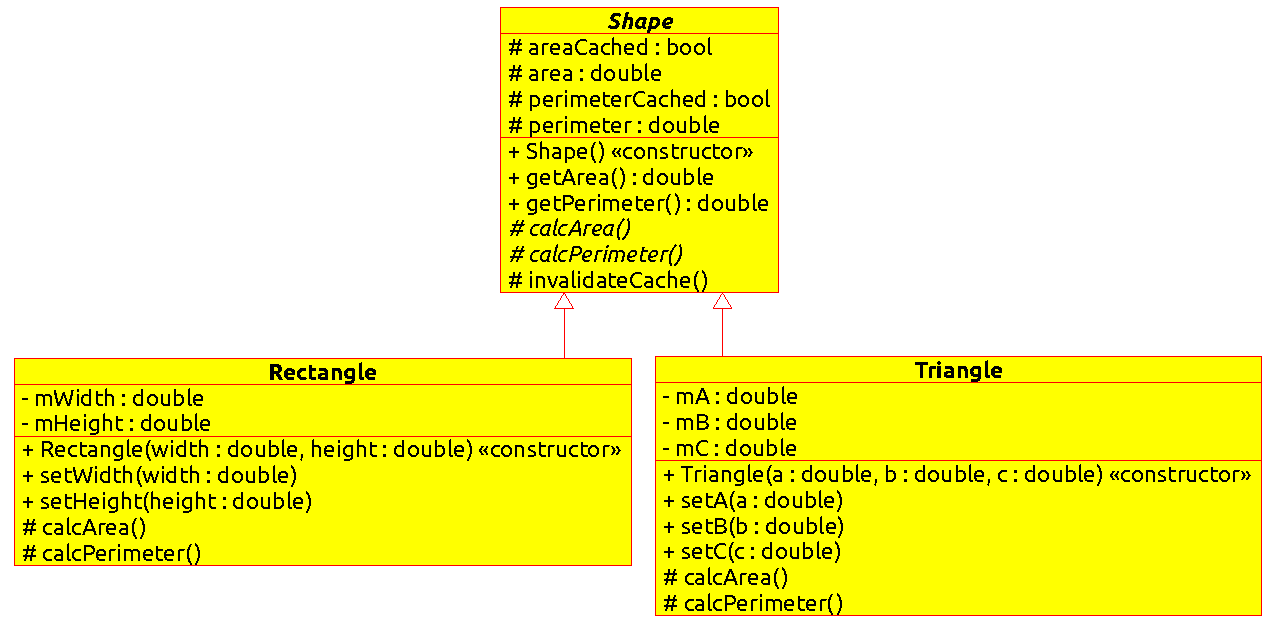
\includegraphics[scale=0.6]{Shape15.eps}
      \end{center}
\end{frame}

\end{document}